% Options for packages loaded elsewhere
\PassOptionsToPackage{unicode}{hyperref}
\PassOptionsToPackage{hyphens}{url}
\PassOptionsToPackage{dvipsnames,svgnames*,x11names*}{xcolor}
%
\documentclass[
  8pt,
  ignorenonframetext,
  dvipsnames]{beamer}
\usepackage{pgfpages}
\setbeamertemplate{caption}[numbered]
\setbeamertemplate{caption label separator}{: }
\setbeamercolor{caption name}{fg=normal text.fg}
\beamertemplatenavigationsymbolsempty
% Prevent slide breaks in the middle of a paragraph
\widowpenalties 1 10000
\raggedbottom
\setbeamertemplate{part page}{
  \centering
  \begin{beamercolorbox}[sep=16pt,center]{part title}
    \usebeamerfont{part title}\insertpart\par
  \end{beamercolorbox}
}
\setbeamertemplate{section page}{
  \centering
  \begin{beamercolorbox}[sep=12pt,center]{part title}
    \usebeamerfont{section title}\insertsection\par
  \end{beamercolorbox}
}
\setbeamertemplate{subsection page}{
  \centering
  \begin{beamercolorbox}[sep=8pt,center]{part title}
    \usebeamerfont{subsection title}\insertsubsection\par
  \end{beamercolorbox}
}
\AtBeginPart{
  \frame{\partpage}
}
\AtBeginSection{
  \ifbibliography
  \else
    \frame{\sectionpage}
  \fi
}
\AtBeginSubsection{
  \frame{\subsectionpage}
}
\usepackage{lmodern}
\usepackage{amssymb,amsmath}
\usepackage{ifxetex,ifluatex}
\ifnum 0\ifxetex 1\fi\ifluatex 1\fi=0 % if pdftex
  \usepackage[T1]{fontenc}
  \usepackage[utf8]{inputenc}
  \usepackage{textcomp} % provide euro and other symbols
\else % if luatex or xetex
  \usepackage{unicode-math}
  \defaultfontfeatures{Scale=MatchLowercase}
  \defaultfontfeatures[\rmfamily]{Ligatures=TeX,Scale=1}
\fi
% Use upquote if available, for straight quotes in verbatim environments
\IfFileExists{upquote.sty}{\usepackage{upquote}}{}
\IfFileExists{microtype.sty}{% use microtype if available
  \usepackage[]{microtype}
  \UseMicrotypeSet[protrusion]{basicmath} % disable protrusion for tt fonts
}{}
\makeatletter
\@ifundefined{KOMAClassName}{% if non-KOMA class
  \IfFileExists{parskip.sty}{%
    \usepackage{parskip}
  }{% else
    \setlength{\parindent}{0pt}
    \setlength{\parskip}{6pt plus 2pt minus 1pt}}
}{% if KOMA class
  \KOMAoptions{parskip=half}}
\makeatother
\usepackage{xcolor}
\IfFileExists{xurl.sty}{\usepackage{xurl}}{} % add URL line breaks if available
\IfFileExists{bookmark.sty}{\usepackage{bookmark}}{\usepackage{hyperref}}
\hypersetup{
  pdftitle={Introduction to Multivariate Regression \& Econometrics},
  pdfauthor={Lecture 8},
  colorlinks=true,
  linkcolor=Maroon,
  filecolor=Maroon,
  citecolor=Blue,
  urlcolor=blue,
  pdfcreator={LaTeX via pandoc}}
\urlstyle{same} % disable monospaced font for URLs
\newif\ifbibliography
\usepackage{color}
\usepackage{fancyvrb}
\newcommand{\VerbBar}{|}
\newcommand{\VERB}{\Verb[commandchars=\\\{\}]}
\DefineVerbatimEnvironment{Highlighting}{Verbatim}{commandchars=\\\{\}}
% Add ',fontsize=\small' for more characters per line
\usepackage{framed}
\definecolor{shadecolor}{RGB}{248,248,248}
\newenvironment{Shaded}{\begin{snugshade}}{\end{snugshade}}
\newcommand{\AlertTok}[1]{\textcolor[rgb]{0.94,0.16,0.16}{#1}}
\newcommand{\AnnotationTok}[1]{\textcolor[rgb]{0.56,0.35,0.01}{\textbf{\textit{#1}}}}
\newcommand{\AttributeTok}[1]{\textcolor[rgb]{0.77,0.63,0.00}{#1}}
\newcommand{\BaseNTok}[1]{\textcolor[rgb]{0.00,0.00,0.81}{#1}}
\newcommand{\BuiltInTok}[1]{#1}
\newcommand{\CharTok}[1]{\textcolor[rgb]{0.31,0.60,0.02}{#1}}
\newcommand{\CommentTok}[1]{\textcolor[rgb]{0.56,0.35,0.01}{\textit{#1}}}
\newcommand{\CommentVarTok}[1]{\textcolor[rgb]{0.56,0.35,0.01}{\textbf{\textit{#1}}}}
\newcommand{\ConstantTok}[1]{\textcolor[rgb]{0.00,0.00,0.00}{#1}}
\newcommand{\ControlFlowTok}[1]{\textcolor[rgb]{0.13,0.29,0.53}{\textbf{#1}}}
\newcommand{\DataTypeTok}[1]{\textcolor[rgb]{0.13,0.29,0.53}{#1}}
\newcommand{\DecValTok}[1]{\textcolor[rgb]{0.00,0.00,0.81}{#1}}
\newcommand{\DocumentationTok}[1]{\textcolor[rgb]{0.56,0.35,0.01}{\textbf{\textit{#1}}}}
\newcommand{\ErrorTok}[1]{\textcolor[rgb]{0.64,0.00,0.00}{\textbf{#1}}}
\newcommand{\ExtensionTok}[1]{#1}
\newcommand{\FloatTok}[1]{\textcolor[rgb]{0.00,0.00,0.81}{#1}}
\newcommand{\FunctionTok}[1]{\textcolor[rgb]{0.00,0.00,0.00}{#1}}
\newcommand{\ImportTok}[1]{#1}
\newcommand{\InformationTok}[1]{\textcolor[rgb]{0.56,0.35,0.01}{\textbf{\textit{#1}}}}
\newcommand{\KeywordTok}[1]{\textcolor[rgb]{0.13,0.29,0.53}{\textbf{#1}}}
\newcommand{\NormalTok}[1]{#1}
\newcommand{\OperatorTok}[1]{\textcolor[rgb]{0.81,0.36,0.00}{\textbf{#1}}}
\newcommand{\OtherTok}[1]{\textcolor[rgb]{0.56,0.35,0.01}{#1}}
\newcommand{\PreprocessorTok}[1]{\textcolor[rgb]{0.56,0.35,0.01}{\textit{#1}}}
\newcommand{\RegionMarkerTok}[1]{#1}
\newcommand{\SpecialCharTok}[1]{\textcolor[rgb]{0.00,0.00,0.00}{#1}}
\newcommand{\SpecialStringTok}[1]{\textcolor[rgb]{0.31,0.60,0.02}{#1}}
\newcommand{\StringTok}[1]{\textcolor[rgb]{0.31,0.60,0.02}{#1}}
\newcommand{\VariableTok}[1]{\textcolor[rgb]{0.00,0.00,0.00}{#1}}
\newcommand{\VerbatimStringTok}[1]{\textcolor[rgb]{0.31,0.60,0.02}{#1}}
\newcommand{\WarningTok}[1]{\textcolor[rgb]{0.56,0.35,0.01}{\textbf{\textit{#1}}}}
\usepackage{graphicx,grffile}
\makeatletter
\def\maxwidth{\ifdim\Gin@nat@width>\linewidth\linewidth\else\Gin@nat@width\fi}
\def\maxheight{\ifdim\Gin@nat@height>\textheight\textheight\else\Gin@nat@height\fi}
\makeatother
% Scale images if necessary, so that they will not overflow the page
% margins by default, and it is still possible to overwrite the defaults
% using explicit options in \includegraphics[width, height, ...]{}
\setkeys{Gin}{width=\maxwidth,height=\maxheight,keepaspectratio}
% Set default figure placement to htbp
\makeatletter
\def\fps@figure{htbp}
\makeatother
\setlength{\emergencystretch}{3em} % prevent overfull lines
\providecommand{\tightlist}{%
  \setlength{\itemsep}{0pt}\setlength{\parskip}{0pt}}
\setcounter{secnumdepth}{-\maxdimen} % remove section numbering

%packages
\usepackage{graphicx}
\usepackage{rotating}
\usepackage{hyperref}

\usepackage{tikz} % used for text highlighting, amongst others
\usepackage{comment}

%title slide stuff
%\institute{Department of Education}
%\title{Managing and Manipulating Data Using R}

%
\setbeamertemplate{navigation symbols}{} % get rid of navigation icons:
\setbeamertemplate{footline}[page number]

%\setbeamertemplate{frametitle}{\thesection \hspace{0.2cm} \insertframetitle}
\setbeamertemplate{section in toc}[sections numbered]
%\setbeamertemplate{subsection in toc}[subsections numbered]
\setbeamertemplate{subsection in toc}{%
  \leavevmode\leftskip=3.2em\color{gray}\rlap{\hskip-2em\inserttocsectionnumber.\inserttocsubsectionnumber}\inserttocsubsection\par
}

%define colors
%\definecolor{uva_orange}{RGB}{216,141,42} % UVa orange (Rotunda orange)
\definecolor{mygray}{rgb}{0.95, 0.95, 0.95} % for highlighted text
	% grey is equal parts red, green, blue. higher values >> lighter grey
	%\definecolor{lightgraybo}{rgb}{0.83, 0.83, 0.83}

% new commands

%highlight text with very light grey
\newcommand*{\hlg}[1]{%
	\tikz[baseline=(X.base)] \node[rectangle, fill=mygray] (X) {#1};%
}
%, inner sep=0.3mm
%highlight text with very light grey and use font associated with code
\newcommand*{\hlgc}[1]{\texttt{\hlg{#1}}}

%modifying back ticks to add grey background
\let\OldTexttt\texttt
\renewcommand{\texttt}[1]{\OldTexttt{\hlg{#1}}}


\begin{comment}

% Font
\usepackage[defaultfam,light,tabular,lining]{montserrat}
\usepackage[T1]{fontenc}
\renewcommand*\oldstylenums[1]{{\fontfamily{Montserrat-TOsF}\selectfont #1}}

% Change color of boldface text to darkgray
\renewcommand{\textbf}[1]{{\color{darkgray}\bfseries\fontfamily{Montserrat-TOsF}#1}}

% Bullet points
\setbeamertemplate{itemize item}{\color{BlueViolet}$\circ$}
\setbeamertemplate{itemize subitem}{\color{BrickRed}$\triangleright$}
\setbeamertemplate{itemize subsubitem}{$-$}

% Reduce space before lists
%\addtobeamertemplate{itemize/enumerate body begin}{}{\vspace*{-8pt}}

\let\olditem\item
\renewcommand{\item}{%
  \olditem\vspace{4pt}
}

% decreasing space before and after level-2 bullet block
%\addtobeamertemplate{itemize/enumerate subbody begin}{}{\vspace*{-3pt}}
%\addtobeamertemplate{itemize/enumerate subbody end}{}{\vspace*{-3pt}}

% decreasing space before and after level-3 bullet block
%\addtobeamertemplate{itemize/enumerate subsubbody begin}{}{\vspace*{-2pt}}
%\addtobeamertemplate{itemize/enumerate subsubbody end}{}{\vspace*{-2pt}}

%Section numbering
\setbeamertemplate{section page}{%
    \begingroup
        \begin{beamercolorbox}[sep=10pt,center,rounded=true,shadow=true]{section title}
        \usebeamerfont{section title}\thesection~\insertsection\par
        \end{beamercolorbox}
    \endgroup
}

\setbeamertemplate{subsection page}{%
    \begingroup
        \begin{beamercolorbox}[sep=6pt,center,rounded=true,shadow=true]{subsection title}
        \usebeamerfont{subsection title}\thesection.\thesubsection~\insertsubsection\par
        \end{beamercolorbox}
    \endgroup
}

\end{comment}

\title{Introduction to Multivariate Regression \& Econometrics}
\subtitle{HED 612}
\author{Lecture 8}
\date{}

\begin{document}
\frame{\titlepage}

\begin{frame}
  \tableofcontents[hideallsubsections]
\end{frame}
\hypertarget{logistics}{%
\section{Logistics}\label{logistics}}

\begin{frame}{Download Data and Open R Script}
\protect\hypertarget{download-data-and-open-r-script}{}

We're going to use GSS and ELS data today. We'll also explore HSLS later
on but we will load the dataset together!

\medskip

\begin{enumerate}
\tightlist
\item
  Download the Lecture 8 PDF and R files for this week

  \begin{itemize}
  \tightlist
  \item
    Place all files in HED612\_S21
    \textgreater\textgreater\textgreater{} lectures
    \textgreater\textgreater\textgreater{} lecture8
  \end{itemize}
\item
  Open the RProject (should be in your main HED612\_S21 folder)
\item
  Once the RStudio window opens, open the Lecture 8 R script by clicking
  on:

  \begin{itemize}
  \tightlist
  \item
    file \textgreater\textgreater\textgreater{} open file\ldots{}
    \textgreater\textgreater\textgreater{} {[}navigate to lecture 8
    folder{]} \textgreater\textgreater\textgreater{} lecture8.R
  \end{itemize}
\end{enumerate}

\end{frame}

\begin{frame}{Outline of next couple weeks}
\protect\hypertarget{outline-of-next-couple-weeks}{}

Today, 3/5/2020:

\begin{itemize}
\tightlist
\item
  Review SER vs SE of \(\hat{\beta_1}\)
\item
  More practice in interpreting Categorical X
\item
  More practice in creating variables in R
\item
  Review requirements for final project
\item
  National Datasets you can use for final project!
\end{itemize}

\medskip

Homework and Reading for 3/17/2021:

\begin{itemize}
\tightlist
\item
  PS\#8 Posted on D2L due 3/17/2020
\item
  Reading:

  \begin{itemize}
  \tightlist
  \item
    TBD
  \end{itemize}
\end{itemize}

\medskip

3/10/2020: Spring Break/Reading Day No Class!

\medskip

03/19/2020:

\begin{itemize}
\tightlist
\item
  OLS Assumptions
\item
  Introduction to Omitted Variable Bias
\item
  Introduction to Multivariate Regression
\end{itemize}

\end{frame}

\hypertarget{difference-between-standard-error-of-hatbeta_1-and-ser}{%
\section{\texorpdfstring{Difference between Standard Error of
\(\hat{\beta_1}\) and
SER}{Difference between Standard Error of \textbackslash hat\{\textbackslash beta\_1\} and SER}}\label{difference-between-standard-error-of-hatbeta_1-and-ser}}

\begin{frame}{Standard Error of \(\hat{\beta_1}\)}
\protect\hypertarget{standard-error-of-hatbeta_1}{}

\begin{itemize}
\item
  Standard error of \(\hat{\beta_1}\) is the \emph{estimated standard
  deviation} of the \emph{error} in measuring it
\item
  We generate Standard error of \(\hat{\beta_1}\) via hypothesis
  testing!

  \begin{itemize}
  \tightlist
  \item
    Hypothesis testing is our attempt to identify variation in a point
    estimate that could be due to sampling (variation that occurs by
    chance from one sample to another) in order to confirm that our
    estimate is ``true'' and did not occur just by random chance! (i.e.,
    statistically significant!)
  \item
    Think of the ``three pictures'':
  \item
    Hypothesis testing about population mean: \(SE(\bar{Y})\) is the
    average distance of a single sample mean \(\bar{Y}\) from the mean
    of sample means \(\bar{Y}_Y\) (mean of sample means = true
    population mean)
  \item
    Hypothesis testing about \(\hat{\beta_1}\): \(SE(\hat{\beta_1})\) is
    the average distance of our sample estimate of the effect of X on Y
    (\(\hat{\beta_1}\)) from the mean of sample estimates of \(\beta_1\)
    (mean of sample estimates = true population \(\beta_1\))
  \end{itemize}
\item
  Our null hypothesis is always \(H_0: \beta_1 = 0\)

  \begin{itemize}
  \tightlist
  \item
    Meaning: the effect of X on Y is really zero once we we take into
    account sampling variability. In other words, any non-zero effect we
    find is because of sampling variability!
  \item
    In causal inference research the null hypothesis is a ``straw man'';
    we want to disprove it.
  \item
    Disproving it would mean that our non-zero effect of X on Y is not
    due to random sampling variability, but is indicative of a real,
    causal relationship!
  \item
    The p-value is the probability that the test statistic for
    \(\hat{\beta_1}\) equals the observed value or a value even more
    extreme than \(\hat{\beta_1}\) if \(H_0\) is true
  \item
    A small p-value disproves the null because it would be so unlikely
    (less than 5\% probability) to find the observed data if \(H_0\)
    were true
  \end{itemize}
\end{itemize}

\end{frame}

\begin{frame}[fragile]{Standard Error of \(\hat{\beta_1}\)}
\protect\hypertarget{standard-error-of-hatbeta_1-1}{}

RQ: What is the effect of hours worked per week (X) on annual income
(Y)?

\begin{itemize}
\tightlist
\item
  If we run
  \texttt{mod1\ \textless{}-\ lm(realrinc\ \textasciitilde{}\ hrs1,\ data=gss)};
  we get a \(\hat{\beta_1}\)=\$455
\item
  Every one hour increase in hours worked per week is associated with a
  \$455 increase in annual income

  \begin{itemize}
  \tightlist
  \item
    Our slope of relationship between hours worked per week (X) and
    annual income (Y) is \$455
  \item
    How do we determine ``how far'' this slope of \$455 estimated from
    one random sample of 2,348 people is from the true population
    estimate for all people in the US?
  \item
    The standard error of \(\hat{\beta_1}\) is the standard deviation of
    the sampling distribution!
  \end{itemize}
\end{itemize}

SE(\(\hat{\beta_1}\))

\begin{itemize}
\tightlist
\item
  Needed to construct Confidence Intervals
\item
  Needed to rule out how much of our estimate is likely attributed to
  random sampling variability and how likely it is that we're generating
  a statistically significant estimate of the true population effect of
  X on Y.
\item
  So, it is really key to allow you to interpret and evaluate your
  regression model.
\end{itemize}

\end{frame}

\begin{frame}{SER}
\protect\hypertarget{ser}{}

\textbf{Standard Error of the Regression (SER)}: A measure of
``model-fit'', in other words the standard deviation of the residuals
\(\hat{u_i}\)

\begin{itemize}
\item
  On average, how far away an actual observed value of Y is from the
  predicted value of Y for a random observation
\item
  Which would have a better SER?
\end{itemize}

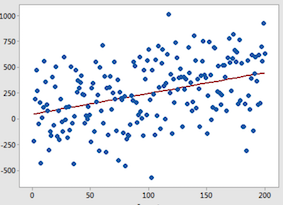
\includegraphics{ser1.png} 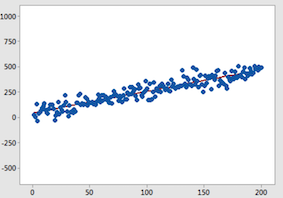
\includegraphics{ser2.png}

\end{frame}

\begin{frame}{SER vs SE(\(\hat{\beta_1}\))}
\protect\hypertarget{ser-vs-sehatbeta_1}{}

\begin{itemize}
\tightlist
\item
  \textbf{Standard error of the regression}

  \begin{itemize}
  \tightlist
  \item
    It's completely determined by your sample data
  \item
    Says nothing about how ``far'' our slope estimates based on our one
    random sample likely are from true population parameters!
  \item
    That's why it's a \textbf{measure of model fit or ``goodness of fit
    measure''}! It tells us how good our line is fitting our ONE random
    sample!
  \item
    High SER tells us that our predictions will often be wrong by a lot;
    but in causal inference research that does not necessarily mean our
    model is bad given some things are hard to predict and we often are
    interested in ``averages''!
  \end{itemize}
\end{itemize}

\medskip

\begin{itemize}
\tightlist
\item
  \textbf{Standard error of \(\hat{\beta_1}\)}

  \begin{itemize}
  \tightlist
  \item
    Is key to determining \textbf{statistical significance} of the
    relationship between X and Y; statistical significance is the
    likelihood that a relationship between two or more variables is
    caused by something other than random chance
  \item
    Requires simulating lots of random samples of \(\hat{\beta_1}\) to
    generate a sampling distribution in which the mean of the sampling
    distribution = true population \(\beta_1\)
  \end{itemize}
\end{itemize}

\end{frame}

\hypertarget{more-practice-on-interpreting-categorical-x}{%
\section{More Practice on Interpreting Categorical
X}\label{more-practice-on-interpreting-categorical-x}}

\begin{frame}{Interpretation of \(\hat{\beta_1}\)}
\protect\hypertarget{interpretation-of-hatbeta_1}{}

\begin{itemize}
\tightlist
\item
  Generic interpretation for \(\hat{\beta_1}\) when X=continuous

  \begin{itemize}
  \tightlist
  \item
    The average effect of a one-unit increase in X is associated with a
    \(\hat{\beta_1}\) change in the value of Y
  \end{itemize}
\item
  Generic interpretation for \(\hat{\beta_1}\) when X= categorical

  \begin{itemize}
  \tightlist
  \item
    the average effect of being {[}specific non-reference category{]} as
    opposed to {[}reference category{]} is associated with a
    \(\hat{\beta_1}\) change in the value of Y
  \end{itemize}
\end{itemize}

\medskip

\begin{itemize}
\tightlist
\item
  General Steps for regression with categorical X

  \begin{itemize}
  \tightlist
  \item
    Identify the categories of X and choose a reference group
  \item
    Create the variable(s) by either

    \begin{itemize}
    \tightlist
    \item
      Creating dummy variables for each group (and leave out the
      reference group dummy); \emph{OR}
    \item
      Use the R shortcut: code all groups into one categorical variable;
      code the reference group as the lowest value (which will be left
      out of the regression automatically by R) OR explicitly tell R
      what the reference category is
    \end{itemize}
  \item
    Write out population regression
  \item
    Write out OLS prediction line with estimates
  \item
    Interpret estimates
  \item
    Predict \(\hat{Y}\) for groups of interest!
  \end{itemize}
\end{itemize}

\end{frame}

\begin{frame}{Example on Interpreting Categorical X}
\protect\hypertarget{example-on-interpreting-categorical-x}{}

RQ: What is the effect of socioeconomic status quartile (X) on reading
score (Y)?

Let's go through each step of the process using the above example!

\end{frame}

\begin{frame}[fragile]{First step: investigate categories of X and
choosing a reference group}
\protect\hypertarget{first-step-investigate-categories-of-x-and-choosing-a-reference-group}{}

The first steps are investigating categories of X and choosing a
reference group and then creating the variable(s) in R

\medskip

``Conceptual'' Process for Creating ``analysis'' variables in R

\begin{enumerate}
\tightlist
\item
  Investigating values and patterns of variables from ``input data''
\item
  Identifying and cleaning errors or values that need to be changed
\item
  Creating ``analysis'' variables
\item
  Checking values of analysis variables against values of input
  variables
\end{enumerate}

\medskip

How to investigate values and patterns of variable from ``input data''
when X=Categorical

\begin{itemize}
\tightlist
\item
  use \texttt{var\_label()} + \texttt{val\_labels()} to check variable
  and value labels (not all variables have labels!)
\item
  use \texttt{count()} to get a frequency count of each category
\item
  use \texttt{count()} + \texttt{is.na()} to explicitly check if there
  are any missing observations
\end{itemize}

\end{frame}

\begin{frame}[fragile]{Creating ``different'' categorical variables and
R code}
\protect\hypertarget{creating-different-categorical-variables-and-r-code}{}

\begin{itemize}
\tightlist
\item
  What if we want to create a dummy variable?

  \begin{itemize}
  \tightlist
  \item
    high\_ses = 1 for respondents in top two quartiles {[}non-reference
    group{]}
  \item
    high\_ses = 0 for respondents in bottom two quartiles {[}reference
    group{]}
  \item
    And true missing observations should be \texttt{NA}
  \item
    always code your reference group as the lowest value!
  \end{itemize}
\end{itemize}

\medskip

Create dummy vars via \texttt{mutate()} + \texttt{ifelse()} {[}My
general process{]}

\begin{itemize}
\tightlist
\item
  Create two \textbf{new variables}
\item
  First new variable will be a ``version 2'' of the input variable that
  codes ``true missing'' (\texttt{NA}) for values -8 in the original
  variable (\texttt{f1ses1qu\_v2})
\item
  Then, I create my analysis variable that is coded via dummy values
  according to reference and non-reference categories above
  (\texttt{ses\_high})
\end{itemize}

Where general syntax is:

\begin{Shaded}
\begin{Highlighting}[]
\NormalTok{ df <-}\StringTok{ }\NormalTok{df }\OperatorTok\StringTok{ }
\StringTok{  }\KeywordTok{mutate}\NormalTok{(}\DataTypeTok{NEWVAR=} 
           \KeywordTok{ifelse}\NormalTok{(OLDVAR}\OperatorTok{+}\NormalTok{CONDITION, value }\ControlFlowTok{if} \OtherTok{TRUE}\NormalTok{, value }\ControlFlowTok{if} \OtherTok{FALSE}\NormalTok{))}
\end{Highlighting}
\end{Shaded}

See R script for example of this process!

\end{frame}

\begin{frame}[fragile]{Creating ``different'' categorical variables and
R code}
\protect\hypertarget{creating-different-categorical-variables-and-r-code-1}{}

\begin{itemize}
\tightlist
\item
  What if we want to create a multi-categorical variable that is very
  similar to the original?

  \begin{itemize}
  \tightlist
  \item
    We'll keep quartiles as they are; highest quartile=4 and lowest
    quartile=1
  \item
    Respondents in top quartiles (2,3,4) {[}non-reference groups{]}
  \item
    Respondents in lowest quartile (1) {[}reference group{]}
  \item
    And true missing observations should be \texttt{NA}
  \item
    always code your reference group as the lowest value!
  \end{itemize}
\end{itemize}

\medskip

When creating a new variable that is ``simple'' (only one input
variable), create it via \texttt{mutate()} + \texttt{recode()}

\begin{itemize}
\tightlist
\item
  You're creating a \textbf{new variable}, not changing the original!
\end{itemize}

Where general syntax is:

\begin{Shaded}
\begin{Highlighting}[]
\NormalTok{df <-}\StringTok{ }\NormalTok{df }\OperatorTok\StringTok{ }
\StringTok{  }\KeywordTok{mutate}\NormalTok{(}\DataTypeTok{NEWVARIABLE =} \KeywordTok{recode}\NormalTok{(OLDVAR,}
                               \StringTok{`}\DataTypeTok{old_value}\StringTok{`}\NormalTok{ =}\StringTok{ }\NormalTok{new_value,}
                               \StringTok{`}\DataTypeTok{old_value}\StringTok{`}\NormalTok{ =}\StringTok{ }\NormalTok{new_value,}
                               \StringTok{`}\DataTypeTok{old_value}\StringTok{`}\NormalTok{ =}\StringTok{ }\NormalTok{new_value,}
                               \StringTok{`}\DataTypeTok{old_value}\StringTok{`}\NormalTok{ =}\StringTok{ }\NormalTok{new_value) )}
\end{Highlighting}
\end{Shaded}

See R script for example of this process!

\end{frame}

\begin{frame}[fragile]{Creating ``different'' categorical variables and
R code}
\protect\hypertarget{creating-different-categorical-variables-and-r-code-2}{}

\begin{itemize}
\tightlist
\item
  What if we want to create a multi-categorical variable that
  incorporates SES and Race/ethnicity?

  \begin{itemize}
  \tightlist
  \item
    POC respondents in high and low SES quartiles, White respondents in
    High SES quartiles {[}non-reference groups{]}
  \item
    White respondents in low SES quartiles {[}reference group{]}
  \item
    And true missing observations should be \texttt{NA}
  \item
    always code your reference group as the lowest value!
  \end{itemize}
\end{itemize}

\medskip

When creating a new variable that is ``complex'' (multiple input
variables), create it via \texttt{mutate()} + \texttt{case\_when()}

\begin{itemize}
\tightlist
\item
  We're creating a \textbf{new variable}, not changing the original!
\end{itemize}

Where general syntax is:

\begin{Shaded}
\begin{Highlighting}[]
\NormalTok{df <-}\StringTok{ }\NormalTok{df }\OperatorTok\StringTok{ }\KeywordTok{mutate}\NormalTok{(}\DataTypeTok{NEWVARIABLE=}\KeywordTok{case_when}\NormalTok{(}
\NormalTok{             OLDVAR }\KeywordTok{CONDTION}\NormalTok{(S)  }\OperatorTok{~}\StringTok{ }\NormalTok{NEWVALUE, }
\NormalTok{             OLDVAR }\KeywordTok{CONDTION}\NormalTok{(S)  }\OperatorTok{~}\StringTok{ }\NormalTok{NEWVALUE, }
\NormalTok{             OLDVAR }\KeywordTok{CONDTION}\NormalTok{(S)  }\OperatorTok{~}\StringTok{ }\NormalTok{NEWVALUE, }
\NormalTok{             OLDVAR }\KeywordTok{CONDTION}\NormalTok{(S)  }\OperatorTok{~}\StringTok{ }\NormalTok{NEWVALUE )) }
\end{Highlighting}
\end{Shaded}

See R script for example of this process!

\end{frame}

\begin{frame}[fragile]{Example on Interpreting Categorical X}
\protect\hypertarget{example-on-interpreting-categorical-x-1}{}

RQ: What is the effect of socioeconomic status quartile (X) on reading
score (Y)?

\medskip

\begin{itemize}
\tightlist
\item
  Identify the categories of X and choose a reference group

  \begin{itemize}
  \tightlist
  \item
    Let's use the cleaned up version of the 4-category SES quartile
    variable
  \item
    Lowest quartile = reference group
  \item
    Second, Third, and Highest Quartile = non-reference groups
  \end{itemize}
\end{itemize}

\medskip

\begin{itemize}
\tightlist
\item
  Create variables

  \begin{itemize}
  \tightlist
  \item
    already done via shortcut (\texttt{sesquart})
  \end{itemize}
\item
  Write out population regression model
\item
  Write out OLS prediction line with estimates
\item
  Interpret estimates
\item
  Predict \(\hat{Y}\) for each quartile!
\end{itemize}

\end{frame}

\hypertarget{final-research-projects-picking-a-research-question}{%
\section{Final Research Projects, Picking a Research
Question}\label{final-research-projects-picking-a-research-question}}

\begin{frame}{You can \textbf{BEGIN} thinking about final projects;
general requirements}
\protect\hypertarget{you-can-begin-thinking-about-final-projects-general-requirements}{}

\begin{itemize}
\tightlist
\item
  Paper must focus on analyzing the effect of one independent variable
  of interest on some outcome variable
\item
  You can work on your own or in groups of two
\item
  Required sections: introduction, literature review, conceptual
  framework, methods (data, sample, analysis), results, discussion
\item
  This is the first draft of a paper; does not need to be perfect in any
  sense!
\item
  Goal is to give you practice with thinking through purpose of each
  section of a paper and developing sections for a particular research
  question
\item
  Students will give conference style presentation of their paper on
  last day of class!
\end{itemize}

\end{frame}

\begin{frame}{Do's and Dont's for final project}
\protect\hypertarget{dos-and-donts-for-final-project}{}

\textbf{Some cautionary ``don'ts''}:

\begin{itemize}
\tightlist
\item
  Don't freak out! Goal is to get some experience/practice! :)
\item
  Don't pick a dataset or research question that is going to require
  substantial effort/time in building an analysis dataset!

  \begin{itemize}
  \tightlist
  \item
    Unless you will be using these data for something other than this
  \end{itemize}
\item
  Do not pick a research question where you attempt to asses an
  intervention using outcome before the intervention in comparison to
  outcome after the intervention (i.e., pre and post tests)

  \begin{itemize}
  \tightlist
  \item
    This requires additional longitudinal modeling methods that we will
    not cover in this course!
  \item
    Start with analyzing the effect of an intervention on an outcome
    that occurs \emph{after} the intervention
  \item
    Need to pick a research question where you have variation in your
    independent variable of interest (e.g., TRIO participants and
    non-TRIO participants) and outcome data across that variation (i.e.,
    GPAs for both participants/non-participants)
  \end{itemize}
\end{itemize}

\medskip

\textbf{Do:}

\begin{itemize}
\tightlist
\item
  Think of this as a pilot study using ``preliminary data''

  \begin{itemize}
  \tightlist
  \item
    I don't care if you get significant results or not
  \item
    I care more that you are learning how to craft the different
    sections of the paper given your research question and getting some
    practice with data management/interpreting results
  \end{itemize}
\item
  Control Variables {[}haven't covered yet!{]}

  \begin{itemize}
  \tightlist
  \item
    Your paper must discuss what variables should be included to avoid
    omitted variable bias (we'll cover this in the next few weeks); but
    your model does not have to actually have ALL OF THEM
  \item
    I don't expect you to have the time to clean and create all these
    and your dataset might not have them
  \end{itemize}
\end{itemize}

\end{frame}

\begin{frame}{Research questions that work and don't work}
\protect\hypertarget{research-questions-that-work-and-dont-work}{}

\begin{itemize}
\tightlist
\item
  Fundamental requirements:

  \begin{itemize}
  \tightlist
  \item
    Must be feasible for your independent variable to be randomly
    assigned in a random experiment
  \item
    Your dependent variable (Y) needs to be continuous or 0/1
  \item
    Your dependent variable (Y) must be measured at a time after your
    independent variable (X) occurs
  \end{itemize}
\end{itemize}

\medskip

\begin{itemize}
\tightlist
\item
  Easiest independent variables that meet this requirement:
  participation in a program/intervention

  \begin{itemize}
  \tightlist
  \item
    Federal programs: TRIO, Head Start
  \item
    Interventions: dropout prevention program, college prep, financial
    literary programs, using ``services'' like Think Tank, Cultural
    Centers, etc.
  \item
    Others: Student Teacher Ratio, type of sanction (diversion vs
    community service)
  \end{itemize}
\end{itemize}

\medskip

Avoid:

\begin{itemize}
\tightlist
\item
  Independent variables that can't be randomly assigned or are hard to
  measure

  \begin{itemize}
  \tightlist
  \item
    Attitudes or ideologies
  \item
    Culture
  \item
    Leadership Style
  \item
    Personal demographics
  \end{itemize}
\end{itemize}

\end{frame}

\begin{frame}{Exception to using personal demographics as X}
\protect\hypertarget{exception-to-using-personal-demographics-as-x}{}

Generally OK to use personal demographics as X when Y variable is
determined by someone else

\begin{itemize}
\tightlist
\item
  Effect of racial identity (X) on the probability of receiving a reply
  to an admissions inquiry (Y)?
\item
  Effect of racial identity (X) on probability of receiving a call back
  job interview (Y)?
\item
  Effect of gender (X) on teacher course evaluations (Y)?
\end{itemize}

\medskip

But these types of questions require really strong control variables!

\begin{itemize}
\tightlist
\item
  Will cover this more once we cover omitted variable bias
\end{itemize}

\end{frame}

\begin{frame}{As an aside: choosing ``good'' research questions}
\protect\hypertarget{as-an-aside-choosing-good-research-questions}{}

Many different ways to determine ``good'' research questions:

\begin{itemize}
\tightlist
\item
  Importance in regards to informing policy and practice:

  \begin{itemize}
  \tightlist
  \item
    What is the effect of offering max pell grant on college completion?
  \end{itemize}
\item
  ``Interesting'' research

  \begin{itemize}
  \tightlist
  \item
    Sometimes ``good'' research questions are of interest to particular
    audiences (researchers, practitioners, etc)
  \item
    EX: Do public universities recruit students in low-income,
    Communities of Color
  \item
    This example doesn't inform policy explicitly; but shows insights
    into the enrollment priorities of admissions offices
  \end{itemize}
\end{itemize}

\medskip

Choosing your research question is hard!

\begin{itemize}
\tightlist
\item
  You can start with your X
\item
  You can start with your Y
\end{itemize}

\end{frame}

\hypertarget{final-research-projects-possible-data}{%
\section{Final Research Projects, Possible
Data}\label{final-research-projects-possible-data}}

\begin{frame}{Educational Longitudinal Survey (ELS)}
\protect\hypertarget{educational-longitudinal-survey-els}{}

\begin{itemize}
\tightlist
\item
  Nationally representative, longitudinal study of 10th graders in 2002
  and 12th graders in 2004
\item
  Students followed throughout secondary and post secondary years
\item
  Surveys of students, their parents, math and English teachers, and
  school administrators
\item
  Student assessments in math (10th \& 12th grades) and English (10th
  grade)
\item
  High school transcripts available for research on course taking
\end{itemize}

\medskip

Possible research questions:

\begin{itemize}
\tightlist
\item
  What is the effect of taking Advanced Algebra in high school on taking
  a remedial math class in college?
\item
  What is the effect of participation in sports in college on timely
  college graduation?
\end{itemize}

\end{frame}

\begin{frame}{Early Childhood Longitudinal Study (ECLS)}
\protect\hypertarget{early-childhood-longitudinal-study-ecls}{}

\begin{itemize}
\tightlist
\item
  Longitudinal study that examines child development, school readiness,
  and early school experiences
\item
  Actually 4 longitudinal data collections:

  \begin{itemize}
  \tightlist
  \item
    Children born in 2001 followed from birth through kindergarten entry
    {[}ECLS-B{]}
  \item
    Kindergarten class of 1998-99 cohort followed from kindergarten
    through the eighth grade {[}ECLS-K{]}
  \item
    Kindergarten class of 2010-11 cohort followed from kindergarten
    through the fifth grade {[}ECLS-K2011{]}
  \item
    {[}Future{]} Kindergarten- class of 2022-23 will be followed from
    kindergarten through eight grade {[}ECLS-K2023{]}
  \end{itemize}
\end{itemize}

\medskip

Possible research questions:

\begin{itemize}
\tightlist
\item
  What is the effect of participating in Head Start on Reading Mastery?
\item
  What is the effect of race on being placed in Special Education (IEP)?
\end{itemize}

\end{frame}

\begin{frame}{High School Longitudinal Study of 2009 (HSLS)}
\protect\hypertarget{high-school-longitudinal-study-of-2009-hsls}{}

\begin{itemize}
\tightlist
\item
  Nationally representative, longitudinal study of 23,000+ 9th graders
  from 944 schools in 2009, with a first follow-up in 2012 and a second
  follow-up in 2016
\item
  Students followed throughout secondary and post secondary years
\item
  Surveys of students, their parents, math and science teachers, school
  administrators, and school counselors
\item
  Assessment in algebraic skills, reasoning, and problem solving for 9th
  and 11th grades
\end{itemize}

\medskip

Possible research questions:

\begin{itemize}
\tightlist
\item
  What is the effect of school having suspension for truancy policy on
  school dropout rates for males?
\item
  What is the effect of participating in Upward Bound on the level of
  college attended?
\end{itemize}

\end{frame}

\begin{frame}{FYI about NCES Datasets}
\protect\hypertarget{fyi-about-nces-datasets}{}

\begin{itemize}
\tightlist
\item
  These datasets have tons of variables!

  \begin{itemize}
  \tightlist
  \item
    It can get overwhelming to try to manage these datasets
  \item
    I will be helping you all through most of this
  \end{itemize}
\item
  These are ``public use'' datasets

  \begin{itemize}
  \tightlist
  \item
    Many variables are removed in order to protect student identity
  \item
    Be sure you're picking variables that ``public use''
  \end{itemize}
\item
  What I will do\ldots.

  \begin{itemize}
  \tightlist
  \item
    I will create R datasets for these surveys
  \item
    But I won't be cleaning individual variables
  \item
    You need to ``clean''/``create analysis'' variables for your
    particular research question
  \end{itemize}
\end{itemize}

\medskip

\begin{itemize}
\tightlist
\item
  You can use primary data or other secondary data sources at your own
  risk!

  \begin{itemize}
  \tightlist
  \item
    Often primary data is more work to manage, so unless this is
    relevant to your dissertation, it may not be worth the effort!
  \item
    I may not be familiar with other secondary datasets; I'll try to be
    as useful as I can!
  \end{itemize}
\end{itemize}

\end{frame}

\end{document}
